\documentclass[border=1cm]{standalone}
\usepackage{tikz}
\usetikzlibrary{math}

% Команда для квадрата
\newcommand\Square[2]{%
    \draw #1 rectangle ++(#2,#2);%
    \fill #1 rectangle ++(#2,#2);%
}

\begin{document}
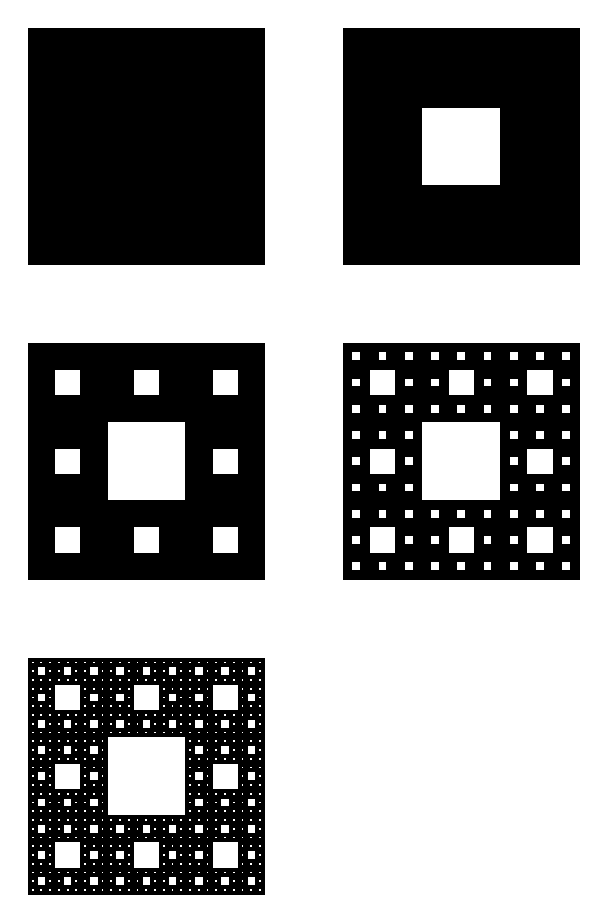
\begin{tikzpicture}
\tikzmath{
    function carpet(\x,\y,\s,\d) {
        if (\d == 0) then {
            {{ \Square{(\x,\y)}{\s}; }};
        } else {
            \newS = \s/3;
            carpet(\x, \y+2*\newS, \newS, \d-1);
            carpet(\x+\newS, \y+2*\newS, \newS, \d-1);
            carpet(\x+2*\newS, \y+2*\newS, \newS, \d-1);
            carpet(\x, \y+\newS, \newS, \d-1);
            carpet(\x+2*\newS, \y+\newS, \newS, \d-1);
            carpet(\x, \y, \newS, \d-1);
            carpet(\x+\newS, \y, \newS, \d-1);
            carpet(\x+2*\newS, \y, \newS, \d-1);
        };
    };
    \S = 3;  
    for \d in {0,...,4} {
        \x = (\S+1)*mod(\d,2);
        \y = int(\d/2)*(\S+1);
        carpet(\x,-\y,\S,\d);
    };
}
\end{tikzpicture}
\end{document}